% !TeX spellcheck = de_DE
\documentclass[ngerman,12pt]{article}

% Packages for Language
\usepackage[ngerman]{babel}
\usepackage[utf8]{inputenc}
\usepackage[T1]{fontenc}
\usepackage[final]{graphicx}
\usepackage{amsmath}
\usepackage{float}
%\usepackage{wrapfig}
\usepackage{caption}
%\usepackage{multirow}
\usepackage{subfig}
\usepackage{hyperref}
\usepackage[german, plain]{fancyref}
\usepackage{afterpage,pdflscape} %%% !!!!!!! CHANGE TO PDFLSCAPE LATER!
\usepackage{varioref}
\usepackage{siunitx}
\usepackage{translator}
\usepackage{listings}
\usepackage{fancyhdr}
\pagestyle{fancy}

%\usepackage{showframe}

\setlength{\headheight}{15.5pt}
\lhead{NAME NAME NAME}
\rhead{\today}
\chead{Numerik Übung 8}


\begin{document}
\lstset{language=Matlab,basicstyle=\ttfamily,columns=fixed}
\subsubsection*{bSpline.m}
\begin{lstlisting}[frame=single]
function [ ys ] = bSpline( xs, m )
ys = zeros(size(xs));
if m == 0
  ys((-0.5 < xs) & (xs <= 0.5))=1;
else
  ys =((xs + 0.5*(m+1))./m).*bSpline(xs+0.5,m-1)+...
       ((0.5*(m+1)-xs)./m).*bSpline(xs-0.5,m-1);
end
end
\end{lstlisting}

\subsubsection*{splineCoeffPeriodic.m}
\begin{lstlisting}[frame=single]
function [ c ] = splineCoeffPeriodic( y, m )
k=floor(m/2);
n=length(y);
Bm = toeplitz(...
  [bSpline(0,m),bSpline(1:k,m),zeros(1,n-2*k-1),...
      bSpline(-(k:-1:1),m)],...
  [bSpline(0,m),bSpline(-(1:k),m),...
      zeros(1,n-2*k-1),bSpline(k:-1:1,m)]);
ca=Bm\y;
c=[ca(n-(k:-1:1));ca;ca((1:k)+1)];
end
\end{lstlisting}
%\filbreak

\subsubsection*{Output}
\begin{figure}[H]
    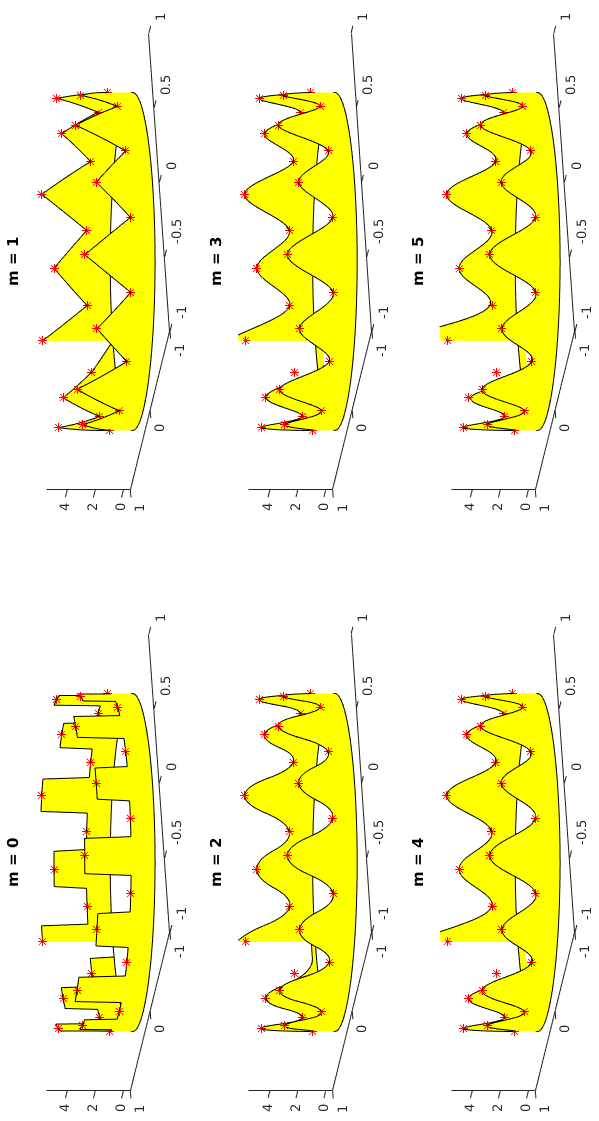
\includegraphics[height=0.93\textheight,keepaspectratio]{result_w_cut_rotated.png}
\end{figure}

\end{document}